\renewcommand*{\arraystretch}{1.1}

\subsection*{Interactive / complex / 14}
\label{section:interactive-complex-read-14}

% change \emph{} to use sans-serif font
\let\oldemph\emph
\renewcommand{\emph}[1]{{\footnotesize \sf #1}}

\renewcommand{\currentQueryCard}{14}
\marginpar{
	\raggedleft
	\vspace{0.22ex}

	\queryRefCard{interactive-complex-read-01}{IC}{1}\\
	\queryRefCard{interactive-complex-read-02}{IC}{2}\\
	\queryRefCard{interactive-complex-read-03}{IC}{3}\\
	\queryRefCard{interactive-complex-read-04}{IC}{4}\\
	\queryRefCard{interactive-complex-read-05}{IC}{5}\\
	\queryRefCard{interactive-complex-read-06}{IC}{6}\\
	\queryRefCard{interactive-complex-read-07}{IC}{7}\\
	\queryRefCard{interactive-complex-read-08}{IC}{8}\\
	\queryRefCard{interactive-complex-read-09}{IC}{9}\\
	\queryRefCard{interactive-complex-read-10}{IC}{10}\\
	\queryRefCard{interactive-complex-read-11}{IC}{11}\\
	\queryRefCard{interactive-complex-read-12}{IC}{12}\\
	\queryRefCard{interactive-complex-read-13}{IC}{13}\\
	\queryRefCard{interactive-complex-read-14}{IC}{14}\\
}


\noindent\begin{tabularx}{\queryCardWidth}{|>{\queryPropertyCell}p{\queryPropertyCellWidth}|X|}
	\hline
	query & Interactive / complex / 14 \\ \hline
%
	title & Trusted connection paths \\ \hline
%
	pattern & \centering 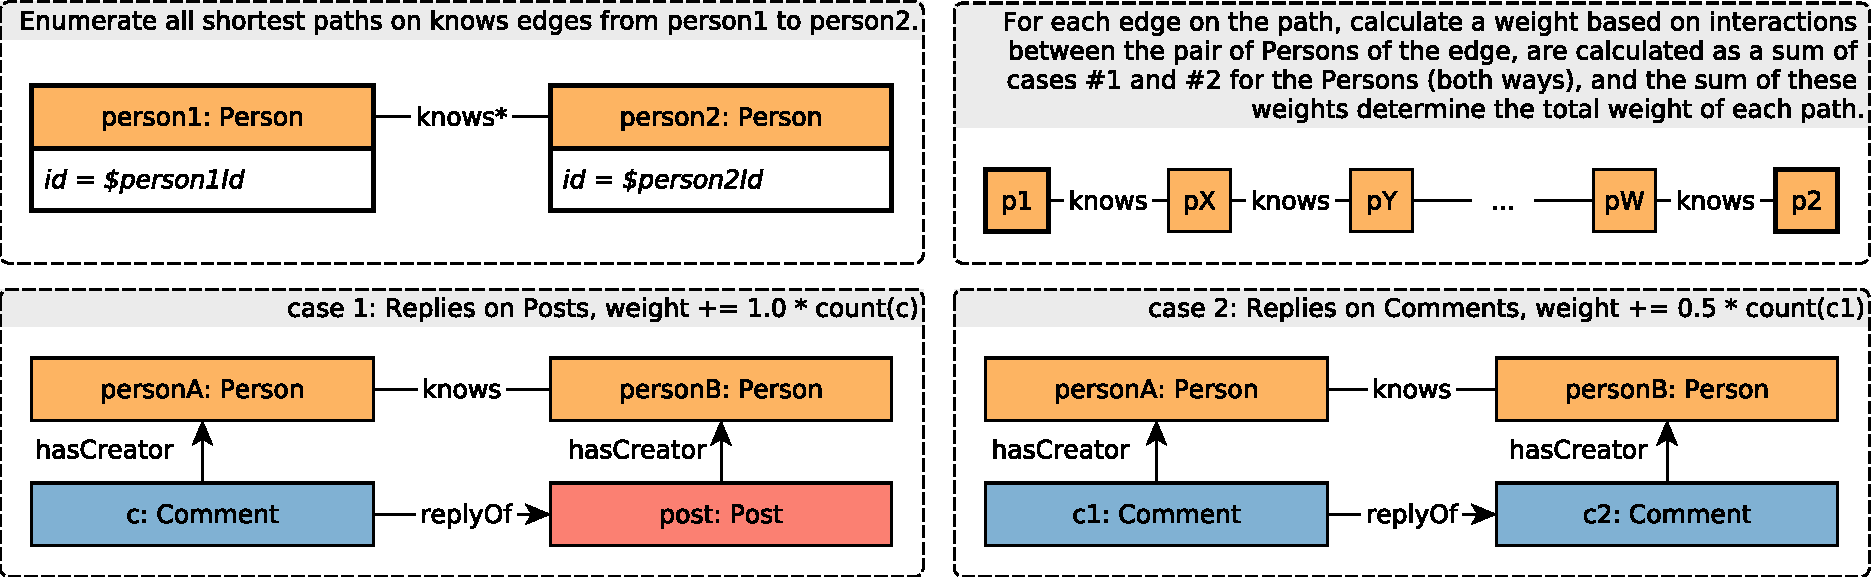
\includegraphics[scale=\patternscale,margin=0cm .2cm]{patterns/interactive-complex-read-14} \tabularnewline \hline
%
	desc. & Given two \emph{Persons}, find all (unweighted) shortest paths between
these two \emph{Persons}, in the subgraph induced by the \emph{knows}
relationship.

Then, for each path calculate a weight. The nodes in the path are
\emph{Persons}, and the weight of a path is the sum of weights between
every pair of consecutive \emph{Person} nodes in the path.

The weight for a pair of \emph{Persons} is calculated based on their
interactions:

\begin{itemize}
\tightlist
\item
  Every direct reply (by one of the \emph{Persons}) to a \emph{Post} (by
  the other \emph{Person}) contributes 1.0.
\item
  Every direct reply (by one of the \emph{Persons}) to a \emph{Comment}
  (by the other \emph{Person}) contributes 0.5.
\end{itemize}

Return all the paths with shortest length, and their weights. Do not
return any rows if there is no path between the two \emph{Persons}.
 \\ \hline
%
	
		params &
		\innerCardVSpace{\begin{tabularx}{\attributeCardWidth}{|>{\paramNumberCell}c|>{\varNameCell}M|>{\typeCell}m{\typeWidth}|Y|} \hline
		$\mathsf{1}$ & person1.id
 & ID
 & \texttt{person1Id}
 \\ \hline
		$\mathsf{2}$ & person2.id
 & ID
 & \texttt{person2Id}
 \\ \hline
		\end{tabularx}}\innerCardVSpace \\ \hline
	
%
	
		result &
		\innerCardVSpace{\begin{tabularx}{\attributeCardWidth}{|>{\resultNumberCell}c|>{\varNameCell}M|>{\typeCell}m{\typeWidth}|>{\resultOriginCell}c|Y|} \hline
		$\mathsf{1}$ & {[}Person.id{]} & {[}ID{]} & C &
				\texttt{personIdsInPath} -- identifiers representing an ordered sequence
of the Persons in the path
 \\ \hline
		$\mathsf{2}$ & weight & 64-bit Float & C &
				\texttt{pathWeight}
 \\ \hline
		\end{tabularx}}\innerCardVSpace \\ \hline
	
%
	
		sort		&
		\innerCardVSpace{\begin{tabularx}{\attributeCardWidth}{|>{\sortNumberCell}c|>{\varNameCell}M|>{\directionCell}c|Y|} \hline
		$\mathsf{1}$ & weight
 & $\desc
$ & The order of paths with the same weight is unspecified
 \\ \hline
		\end{tabularx}}\innerCardVSpace \\ \hline
	%
	%
	CPs &
	\multicolumn{1}{>{\raggedright}l|}{
		\chokePoint{3.3}, 
		\chokePoint{7.2}, 
		\chokePoint{7.3}, 
		\chokePoint{8.1}, 
		\chokePoint{8.6}
		} \\ \hline
	%
	relevance &
		\footnotesize This query looks for a variable length path, starting at a given *Person* and finishing at an another given *Person*. This is a more complex query as it not only requires computing the path length, but returning it and computing a weight. To compute this weight one must look for smaller sub-queries with paths of length three, formed by the two *Persons* at each step, a *Post* and a *Comment*.
 \\ \hline%
\end{tabularx}
\queryCardVSpace

% change \emph back to the old one
\let\emph\oldemph